% huscs, N=32*32*32, numThreadsPerLocale=1,2,3,..,8, step=1
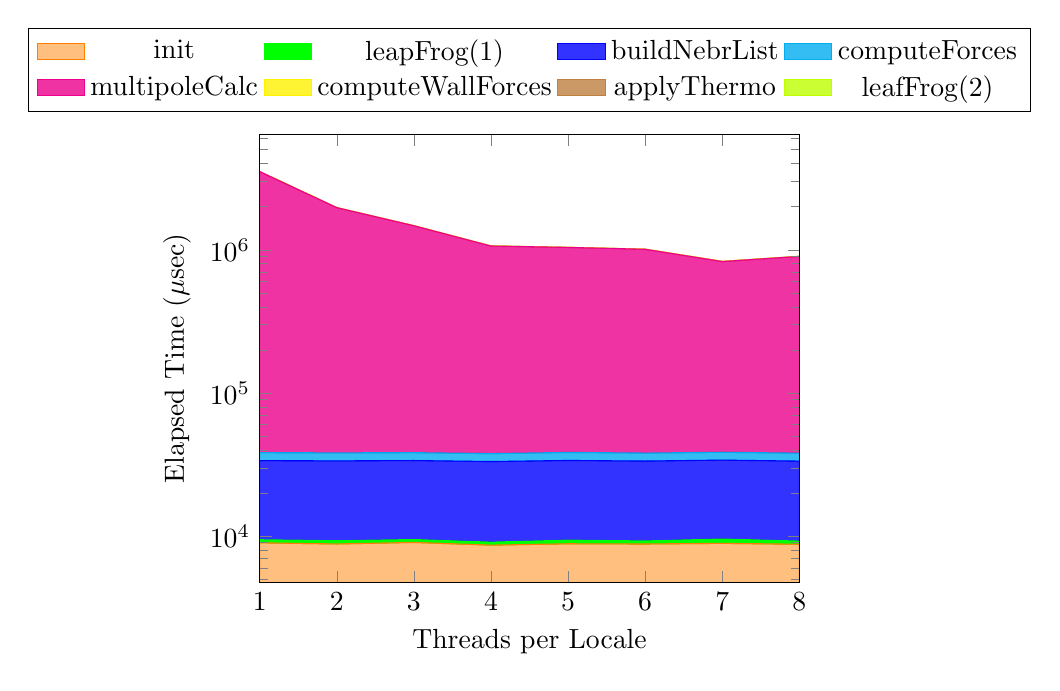
\begin{tikzpicture}
\begin{axis}[
  stack plots=y, area style, enlarge x limits=false,
  ymode=log,
  ylabel=Elapsed Time ($\mu$sec),
  xmin=1, xmax=8, xtick={1, 2, 3, 4, 5, 6, 7, 8},
  xlabel=Threads per Locale,
  legend style={at={(0.5, 1.05)}, anchor=south, legend columns=4}]
\addplot[orange, fill=orange, fill opacity=0.5] coordinates % init
  {(1, 8989) (2, 8825) (3, 9045) (4, 8658) (5, 8850) (6, 8821) (7, 8914) 
   (8, 8783)} \closedcycle;
\addplot[green, fill=green] coordinates % leapFrog(1)
  {(1, 454) (2, 468) (3, 426) (4, 425) (5, 530) (6, 440) (7, 637) (8, 457)}
  \closedcycle;
\addplot[blue, fill=blue, fill opacity=0.8] coordinates % buildNebrList
  {(1, 24268) (2, 24276) (3, 24282) (4, 24134) (5, 24417) (6, 24213) (7, 24434) 
   (8, 24207)} \closedcycle;
\addplot[cyan, fill=cyan, fill opacity=0.8] coordinates % computeForce
  {(1, 4612) (2, 4618) (3, 4564) (4, 4528) (5, 4653) (6, 4581) (7, 4567) 
   (8, 4549)} \closedcycle;
\addplot[magenta, fill=magenta, fill opacity=0.8] coordinates % multipoleCalc
  {(1, 3480480) (2, 1932990) (3, 1434660) (4, 1025450) (5, 1000760) 
   (6, 970789) (7, 789904) (8, 861565)} \closedcycle;
\addplot[yellow, fill=yellow, fill opacity=0.8] coordinates % computeWallForce
  {(1, 727) (2, 840) (3, 738) (4, 659) (5, 509) (6, 619) (7, 811) (8, 450)}
  \closedcycle;
\addplot[brown, fill=brown, fill opacity=0.8] coordinates % applyThermo
  {(1, 647) (2, 724) (3, 798) (4, 690) (5, 670) (6, 679) (7, 906) (8, 649)}
  \closedcycle;
\addplot[lime, fill=lime, fill opacity=0.8] coordinates % leapFrog(2)
  {(1, 233) (2, 380) (3, 399) (4, 340) (5, 335) (6, 364) (7, 447) (8, 334)}
  \closedcycle;
\legend{init, leapFrog(1), buildNebrList, computeForces, multipoleCalc,
    computeWallForces, applyThermo, leafFrog(2)},
\end{axis}
\end{tikzpicture}
